\documentclass[conference]{IEEEtran}
\hyphenation{op-tical net-works semi-conduc-tor}

\usepackage{float}
\usepackage[pdftex]{graphicx}
\usepackage[export]{adjustbox}
\graphicspath{{./figures/}}
\usepackage[sort, numbers]{natbib}
\setcitestyle{square}
\usepackage[table]{xcolor}
\usepackage{tikz}
\usepackage{amsmath}
\usepackage{listings}
\usepackage{color}


% Custom colors
\definecolor{navyblue}{RGB}{31,73,125}
\definecolor{burgundy}{rgb}{0.5, 0.0, 0.13}
\definecolor{lightgray}{rgb}{.6,.6,.6}
\definecolor{darkgray}{rgb}{.2,.2,.2}


\lstdefinelanguage{JavaScript}{
  keywords={typeof, new, true, false, catch, function, return, null, catch, switch, var, if, in, while, do, else, case, break},
  keywordstyle=\color{lightgray}\bfseries,
  ndkeywords={class, export, boolean, throw, implements, import, this},
  ndkeywordstyle=\color{darkgray}\bfseries,
  identifierstyle=\color{black},
  sensitive=false,
  comment=[l]{//},
  morecomment=[s]{/*}{*/},
  commentstyle=\color{lightgray}\ttfamily,
  stringstyle=\color{burgundy}\ttfamily,
  morestring=[b]',
  morestring=[b]"
}

\lstset{
   language=JavaScript,
   backgroundcolor=\color{white},
   extendedchars=true,
   basicstyle=\footnotesize\ttfamily,
   showstringspaces=false,
   showspaces=false,
   numbers=none,
   numberstyle=\footnotesize,
   numbersep=9pt,
   tabsize=2,
   breaklines=true,
   showtabs=false,
   captionpos=b
}


% Scientific notation
\providecommand{\e}[1]{\ensuremath{\times 10^{#1}}}


\begin{document}

\title{Rotation Curve Modeler \\ \Large{A Modeling and Simulating Tool for Arbitrary Galaxies}}


\author{\IEEEauthorblockN{Robert Moss\IEEEauthorrefmark{1}, Alex Clement\IEEEauthorrefmark{2}, Dr. James G. O'Brien \IEEEauthorrefmark{3}, and Mohammed Anwaruddin\IEEEauthorrefmark{4}}
\IEEEauthorblockA{Department of Computer Science and Networking\\
Wentworth Institute of Technology\\
Boston, MA 02115\\
mossr@wit.edu\IEEEauthorrefmark{1}, 
clementa1@wit.edu\IEEEauthorrefmark{2}, 
obrienj10@wit.edu\IEEEauthorrefmark{3},
anwaruddinm@wit.edu\IEEEauthorrefmark{4}}}


\maketitle

\begin{abstract}
%\boldmath
%An abstract is a brief summary of a research article, thesis, review, conference proceeding or any in-depth analysis of a particular subject or discipline, and is often used to help the reader quickly ascertain the paper's purpose.

The development of galaxy models can be tedious and complex. It's also very difficult to sift through peer-reviewed articles to collect data that astronomers have published. Here, we present solutions to these problems with a Rotation Curve Modeler, to model arbitrary galaxies, a Scholarly Observed Celestial Measurements database, to house all the galactic data in a central location, and a Rotation Curve Simulation, to simulate the spin of star clusters around the center of a galaxy.
\end{abstract}


\begin{IEEEkeywords}
galaxy, rotation curve, modeling, simulating, astrophysics, computer science.
\end{IEEEkeywords}


\IEEEpeerreviewmaketitle



\section{Introduction}
In order to model galaxies, astrophysicists would use programs like MATLAB or Mathematica, but there doesn't exist a singular tool to expedite this process in a universal format. The Rotation Curve Modeler (RoCM) serves as this tool to model the rotation of star clusters around the center of a galaxy. Aiding in finding alternate theories to dark matter, it's purpose is to test all existing galactic models against the observational data for the specified galaxy. With observable data from astronomers as the input, any arbitrary galaxy can be imported into the tool. The tool will plot the data and models together, and enable users to import their own galactic models to test against existing theories. Parameter value sliders allow users to control free fitting parameters within the models with real-time visual feedback in the generated graph. This way, each model can be finely tuned to the data, given that the altered parameter value is within the accepted range provided by the astronomers.


\section{Problem}

\subsection{The Rotation Curve Problem}
The physicist Fritz Zwicky working in 1933 for the California Institute of Technology observed the red shift of star clusters within galaxies and stated that the expected velocity was entirely off. The purposed theory was that a matter invisible to the eye -- dark matter -- was in need to account for missing mass that would otherwise hold the clusters together \cite{zwicky}. He proposed that there were ``faint galaxies and diffused gas" that filled in this void \cite{zwicky}. It was later confirmed that such gas was indeed within the galaxy, and as telescopes moved from optical to radio telescopes, the fidelity was high when measuring the amount of gas thanks to the success of spectroscopy.  Although we can now account for this ``missing mass'', many years of evidence has shown that the amount from gas was no where near the volume that was missing in the overall observation. 

Later in the 1970's, Vera Rubin and her colleague, Kent Ford, worked with a new spectrograph that could observe the rotation velocity of spiral-galaxies with incredible accuracy; in both the optical and radio bands \cite{rubin1980}. Upon further research, they concluded that the stars were moving with a uniform velocity around the center of the galaxies, rather than gradually declining in velocity further out (as predicted by general relativity).  Moreover, as their observations advanced, the uniform velocity seemed to trend across all sizes and shapes of galaxies, which would rule out effects of star formation and or galactic evolution. Their findings brought along much speculation.  Since at its heart, the predicted velocity $v$ for the star clusters is a function of only two observational parameters, the distance from the galactic center and the mass of the galaxy. It was realized that if there was invisible mass in the outer regions of galaxies, the prediction and data could be reconciled. This missing factor that increased the predicted velocity is highly thought to be dark matter, yet the true answer is still a mystery. 

%The rotation curve problem has been around for almost a century. Since it's origin, theories have surfaced that claim to solve it. RoCM was built for the purpose of comparing the theories that attempt to solve the ``missing mass'' problem in galaxy rotation curves.

\subsection{Parameter Fitting for Models}
Each galaxy has a set of parameters that may be used as model inputs: 
\begin{table}[h]
	\centering
	\normalsize
	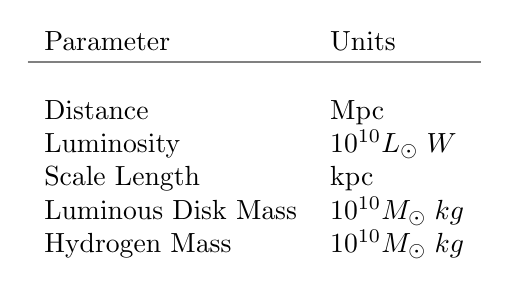
\begin{tikzpicture}
	\node[fill=white,inner sep=0pt] 
	{\rowcolors{1}{white}{white}
		\begin{tabular}{ l l }
		Parameter & Units \\
		\arrayrulecolor{gray}\hline
		\arrayrulecolor{gray}\hline
		&\\
		Distance & Mpc \\
		Luminosity & $10^{10} L_{\odot} \; W$\\
		Scale Length & kpc\\
		Luminous Disk Mass & $10^{10} M_{\odot} \; kg$\\
		Hydrogen Mass & $10^{10} M_{\odot} \; kg$\\
		
		\end{tabular}
	};
	\end{tikzpicture}
\end{table}

Due to the nature of the measurements, astronomers always provide a range for observed parameters. Each galaxy has an accepted range for the number of stars, $N^*$, which is calculated as a ratio of the luminous disk mass over solar mass,
\begin{equation}
N^* = \frac{M_{disk}}{M_{\odot}}.
\end{equation}

\subsubsection{General Relativity}

Referenced from \cite{mannheim}, the normalization parameter, $N^*$, scale length, $R_0$, Schwarzschild radius, $\beta^*$, and the speed of light, $c$, are used in general relativity to model a galaxy's rotation velocity as a function of galactocentric distance, $R$, in the form
\begin{equation}
v_{GR}(R) = \sqrt{\frac{N^*\beta^*c^2R^2}{2R^3_0}F_b}
\end{equation}
where the bessel functions $I_0$, $I_1$, $K_0$, and $K_1$ are used to formulate the curve
\begin{equation}
F_b = \left[I_0\left(\frac{R}{2R_0}\right)K_0\left(\frac{R}{2R_0}\right)-I_1\left(\frac{R}{2R_0}\right)K_1\left(\frac{R}{2R_0}\right)\right].
\end{equation}
It is assumed that each parameter is fixed (other than the input $R$). But since these fixed parameters have an accepted range, it's difficult to alter them and see the behavior of the model. 


\subsubsection{Lambda Cold Dark Matter}
An issue when modeling galaxies is how to best adjust free parameters like $N^*$. Some models have more free parameters than others, all dictated by the theory. The $\Lambda CDM$ theory states that each galaxy has two unobservable parameters, namely the spherical dark matter density, $\sigma_0$, and the dark matter halo radius, $r_0$. As described by \cite{mannheim}, the $\Lambda CDM$ rotation velocity contribution
\begin{equation}
v_{dark}(R) = \sqrt{4\pi\beta^*c^2\sigma_0\left[1-\frac{r_0}{R}\text{arctan}\left(\frac{R}{r_0}\right)\right]}
\end{equation}
is summed with the general relativity contribution to produce a total dark matter rotation velocity of 
\begin{equation}
v_{total}(R) = \sqrt{v_{GR}^2 * v_{dark}^2}.
\end{equation}

In order for $\Lambda CDM$ to work, $\sigma_0$ and $r_0$ have to be fit to the data using a $\chi^2$ test against $v_{total}$. The two free parameters effectively shape the modeled rotation curve to make it precisely fit the data. The problem with parameter fitting is that it's time consuming and can be tough to initialize minimum and maximum ranges without any empirical evidence to suggest a initial value range. To expedite this process, RoCM provides parameter fitting sliders to quickly and visually test each parameter value in the models.

\subsubsection{Conformal Gravity}
Starting with the principle equations of GR, conformal gravity deems to replace GR, but allows it to stay true under certain scales \cite{mannheim}. The intent of GR wasn't for galaxies and the universe as a whole, hence it works perfectly for solar systems, because that's exactly what it was meant for. The motivation for GR's discovery was the need to predict the movement of the planets because the current physics could not. GR replaced Newtonian physics, yet it still allowed Newtons laws to remain true under certain scales. For the same motivation as GR, conformal gravity encompasses the scales of galaxies to explain the interactions between these astronomical objects. 

Not intended to solve the rotation curve problem, conformal gravity seeks to formulate an equally good theory of gravity that is more inclusive than GR. Conformal gravity starts from the first principles of GR, and obeys them throughout. Three additional terms to the GR equation have been appended, $\gamma^*$, $\gamma_0$, and $\kappa$ \cite{mannheim}. These constants include missing feasible physical parameters that Einstein didn't need in order for him to model the solar system. Now that physicists need to model objects at a greater scale, the parameters that were initially scrapped from the theory of general relativity have now been added back in.

The three terms are related by this equality: $\kappa < \gamma_0 < \gamma^*$ \cite{mannheim}. The first term, $\gamma^*$, is a matter inclusive term. Accounting for missing matter in the general relativity formulation, this local matter term has a similar strength to the general relativity term. A global term, $\gamma_0$, includes the matter from the rest of the universe. This linear factor calculates the pull of other galaxies in the universe, because a uniformly separated universe cannot be assumed. The last parameter, and the smallest, $\kappa$ is an inhomogeneity term. The overestimation of matter within the galaxy can be thought of as counting mass that is not within the localized collection of matter, in our case a galaxy. As described by \cite{mannheim}, the final rotation velocity function derived from conformal gravity is given by
\begin{equation}
v_{CG}(R) = \sqrt{\genfrac{}{}{0pt}{}{v_{GR}^2+\frac{N^*\gamma^*c^2R^2}{2R_0}I_1\left(\frac{R}{2R_0}\right)K_1\left(\frac{R}{2R_0}\right)}{+\frac{\gamma_0c^2R}{2}-\kappa c^2R}}
\end{equation}
where the constants are
\begin{equation*}
\begin{split}
\gamma^*=5.42\e{-41} {\rm cm}^{-1}, \\ 
\gamma_0=3.06\e{-30} {\rm cm}^{-1}, \\ 
\text{and}\; \kappa=9.54\e{-54}~{\rm cm}^{-2}.
\end{split}
\end{equation*} 

These small terms exist only at certain scales. This allows conformal gravity to scale down to the solar system, making the three additional terms negligible. GR has the ability to scale down to obey Newtonian physics. Thus, by transitivity, conformal gravity encompasses not only GR, but Newtonian laws of motion as well.

\subsubsection{Bulge contribution}

It can be tough to model the center bulge of stars within a galaxy. This formula from \cite{mannheim} uses the number of stars in the bulge, $N^*_b$, and bulge scale length, $t$, to derive the bulge contribution of

\begin{equation}
v_{bulge}(R) = \sqrt{\frac{2 N^*_b\beta^* c^2}{\pi R} \int_0^{R/t} dz\; z^2K_0(z)}.
\end{equation}

Not every galaxy includes a bulge, thus RoCM provides a means to turn on and off the bulge contribution.

\subsection{Scholarly Observed Celestial Measurements}
Researchers must first sift through peer-reviewed articles and gather galactic data one-by-one before modeling a galaxy. To minimize the time astrophysicists gather data, SOCM was created. SOCM is a public database that serves as a central repository for galactic parameters and observed velocity data. The database can also be used as an API for researchers. Initially, SOCM is comprised of 112 galaxies, including the peer-reviewed galactic parameters and measurements of star velocities contained within. 
       
The idea is for astronomers to submit new measurements to the SOCM administrator for approval. Thus creating a single means of distributing validated measurements of hundreds of galaxies. The input data sent to RoCM is housed within SOCM. This way, if new galaxies get submitted and accepted, RoCM will always have the most up-to-date data that is provided. Programmers may also pull from the SOCM API to use the data for other applications other than rotation curve modeling.

\subsection{Abbreviations and Acronyms}
\begin{itemize}
		\item Rotation Curve Modeler (RoCM) is a tool to model galaxies with different theories.
		\item Scholarly Observed Celestial Measurements (SOCM) centralizes the astronomers observational data into a single database.
		\item Rotation Curve Simulation (RoCS) visualizes the spin of the modeled galaxy.				\item Application Programming Interface (API) explains how software components interact.
		\item Data Driven Documents (D3) is a JavaScript library for data visualization.
		\item Scalable Vector Graphics (SVG) serve as a loss-less graphics format.
		\item Comma-Separated Values (CSV) is a row and column based file format to save data.
        \item Kiloparsecs (kpc) used as the x-axis equates to 3.09\e{19} meters.
        \item Megaparsecs (Mpc) equates to 1000 kpc.
        \item Solar luminosity ($L_{\odot}$) is the brightness of our sun in watts (W).
        \item Solar mass ($M_{\odot}$) is the mass of our sun in kilograms (kg). 
        \item General Relativity (GR) is the theory purposed by Albert Einstein that dictates the interaction of objects in spacetime.
        \item Lambda Cold Dark Matter ($\Lambda CDM$) is the current standard theory for modeling galaxies.
     	\item Conformal Gravity (CG) is an alternate theory to gravity developed by Philip Mannheim and James G. O'Brien.
        \item Chi squared ($\chi^2$) test is a statistical mechanism to find the goodness of fit for experimental data verses observational data.
        
\end{itemize}

\section{Solution}

RoCM seeks to bring together the equations described above, and create a workstation for astrophysicists to quickly and easily model galaxies. The tool consists of 6 major components that all contribute to the powerful functionality we've provided in RoCM:
\begin{enumerate}
       \item The SOCM table drop down for easy access to the database (to select galaxies to plot or download)
       \item The rotation velocity over galactocentric distance graph to plot models against collected data
       \item Parameter sliders to manipulate values within galactic models (for parameter fitting purposes)
       \item A workstation for users to import custom parameters and user defined models to graph
       \item A way to visualize the simulation of the rotation curve (RoCS)
       \item A section for users to import their models in LaTeX format (for better understanding the behavior of parameters within each equation). 

\end{enumerate}



\subsection{Accessing the SOCM database from RoCM}
Figure \ref{socm_fig} shows the table of galactic data that is generated from the SOCM database. The user can sort by value, or search within the table to select a galaxy they would like to plot. The user can also download the parameter and velocity data of the galaxy in a CSV format. The Milky Way data came from \cite{kundu} and \cite{sofue}. The rest of the data included in SOCM came from \cite{mannheim}. 


\subsection{Curve Plot for Rotation Velocity}
\begin{figure}[h!]
\centering
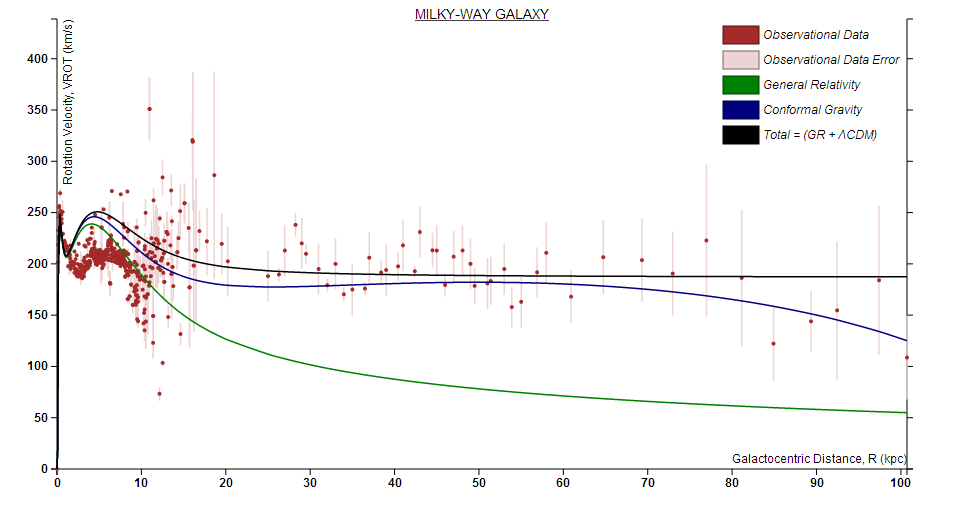
\includegraphics[width=3in, frame]{MILKY-WAY-PLOT2}
\caption{The plotted GR, CR, total $\Lambda CDM$ models over the observational data for the Milky Way (generated from RoCM).}
\label{milkywayplot}
\end{figure}
The main focus of RoCM is the curve plotting tool. Each galactic model is provided in the legend and can be displayed if clicked. The Milky Way's rotation curve can be seen in Figure \ref{milkywayplot}. To see a full screen-shot of the main RoCM page, see Figure \ref{rocm_fig}. You can see the $\chi^2$ table for each model (Figure \ref{chi_fig}) as well as a table of the current parameter values that can be directly edited via the input text box in Figure \ref{param_table_fig} or the parameter sliders drop down (shown in Figure \ref{slider_fig}). 

\begin{figure}[h!]
\centering
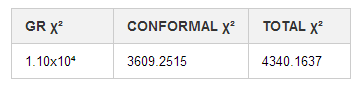
\includegraphics[width=2.5in]{MILKY-WAY-CHI}
\caption{The $\chi^2$ table for the Milky Way galaxy.}
\label{chi_fig}
\end{figure}

Having the $\chi^2$ value presented to the user shows the goodness of fit for each model. We implemented a $\chi^2$ variance because the observational data contains errors, $\mu$, and can be tested with
\begin{equation}
\chi^2 = \sum \frac{(O-E)^2}{\mu^2}
\end{equation} 
where $O$ is the observed data and $E$ is the experimental data (or model data). 

\begin{figure}[h!]
\centering
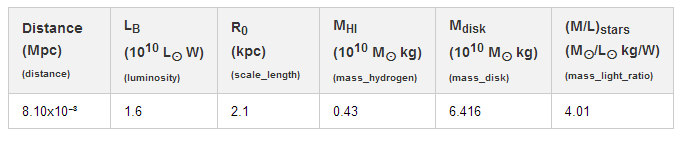
\includegraphics[width=3.5in]{MILKY-WAY-PARAMS}
\caption{The mutable parameters table for the Milky Way galaxy.}
\label{param_table_fig}
\end{figure}

\subsection{Parameter Fitting Sliders}

The power of RoCM lies within these parameter sliders. The user can adjust the minimum and maximum of the parameters and slide the bar to see the how the changes effect the curves on the plot. This responsive visualization helps aid in understanding how each parameter behaves in the theories that use it.

\begin{figure}[h!]
\centering
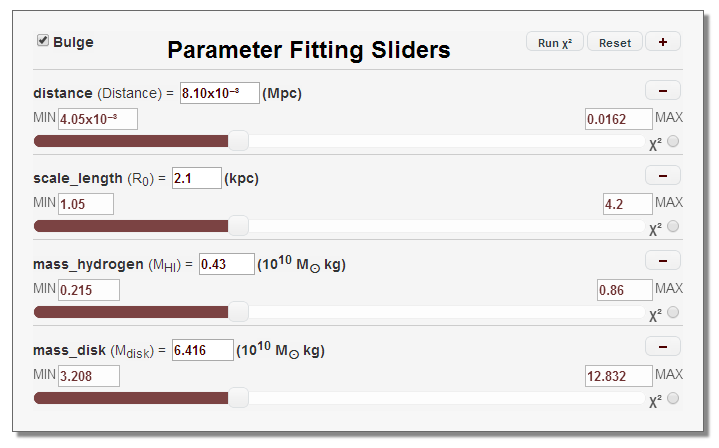
\includegraphics[width=3.5in]{paramslider2}%-full
\caption{Parameter fitting sliders with min and max values.}
\label{slider_fig}
\end{figure}


\subsection{User Defined Models and Parameters}
The included models, namely GR, $\Lambda CDM$, and CG aren't the only theories that model galaxies. Thus, users have the ability to write a model in JavaScript to import directly into RoCM. The User Defined Model workbench (Figure \ref{udm}) opens RoCM up for any and all models that want to be compared against each other. The function should be in the form:
\begin{lstlisting}
function MODELNAME(R){
  var rotation_velocity;
  // The implemented JavaScript model
	
  return rotation_velocity; 
}
\end{lstlisting}


There exist several JavaScript objects that the user can benefit from. 
\subsubsection{PARAMS}
The main parameter object holds all the information of the current parameters. Within your custom model, you can access the parameter via
\begin{lstlisting}
// Returns value * multiplier
PARAMS.get("parameter_name"); 
// Returns the value
PARAMS.getValue("parameter_name"); 
// Returns the multiplier
PARAMS.getMultiplier("parameter_name"); 
// Returns the units
PARAMS.getUnits("parameter_name"); 

// Returns the original value * multiplier
PARAMS.getOriginal("parameter_name"); 
// Returns the original value
PARAMS.getOriginalValue("parameter_name"); 
\end{lstlisting}
where ``parameter\_name'' is the short name of the parameter (defined in Appendix \ref{short_name}). Each parameter within the PARAMS object is a custom Param class. The Param class takes five arguments in the constructor:
\begin{lstlisting}
Param(value, units, multiplier, min, max)
\end{lstlisting}
where the value is the given value as seen in the tables, the units is a string that can be use HTML formatting (for superscripts and subscripts), a multiplier for large numbers (ex: mass\_disk has a multiplier of $10^{10} M_{\odot}$, or 1.99\e{40}), the minimum value for the slider, and the maximum value for the slider. New parameters can be added via the 'Add new parameters' button in the User Defined Model section.


\subsubsection{CONST}
This object holds the available constants:
\begin{lstlisting}
// Speed of light
CONST.get("c");
CONST.get("speed_of_light");

// Solar mass
CONST.get("Mo");
CONST.get("solar_mass");

// Solar luminosity
CONST.get("Lo");
CONST.get("solar_luminosity");

// Gravitational constant
CONST.get("G");
CONST.get("gravitational_constant");

// Schwarzschild radius
CONST.get("B*");
CONST.get("schwarzschild_radius");
\end{lstlisting}

\subsubsection{CONVERT}
This object holds the available conversion functions:
\begin{lstlisting}
pc_to_kpc
Mpc_to_kpc
kpc_to_Mpc
kpc_to_pc
kpc_to_km
km_to_kpc
km_to_cm
km_to_m
cm_to_kpc
cm_to_km
// GeV/cm^3 to kg/km*s^2
GeVcm3_to_kgkms2
arcsec_to_degree
degree_to_arcsec
rad_to_deg
deg_to_rad

// They can be used via
CONVERT.kpc_to_km(kpc);
\end{lstlisting}

\subsubsection{GMODEL}
Most of the theories rely on GR as a basis to formulate upon. Thus, the GMODEL object can be called from the custom models to access the already implemented galactic models with $R$ as the input:
\begin{lstlisting}
GMODEL.GR(R);
GMODEL.DARK(R);
GMODEL.TOTAL(R);
GMODEL.CONFORMAL(R);
\end{lstlisting}

\subsubsection{BULGE}
The bulge contribution can be calculated via:
\begin{lstlisting}
BULGE(R);
\end{lstlisting}


\subsection{Rotation Curve Simulation}

The Rotation Curve Simulation (RoCS) provides a way to visualize the spin of the galaxy in question. The user can simulate either just the observational data, or a specified model against the data. The color scale represents the relative {\color[HTML]{EA051C} minimum} and {\color[HTML]{1AAF3A} maximum} velocity for the stars around the center of the galaxy. The scale helps recognize when the rotation curve simulation of a model doesn't match up with the observational data.

The NGC-2403 galaxy predicted with GR and CG plotted within RoCM in Figure \ref{ngc2403plot} shows the GR curve starts to gradually decline as the CG curve stays consistent with the data.

\begin{figure}[h!]
\centering
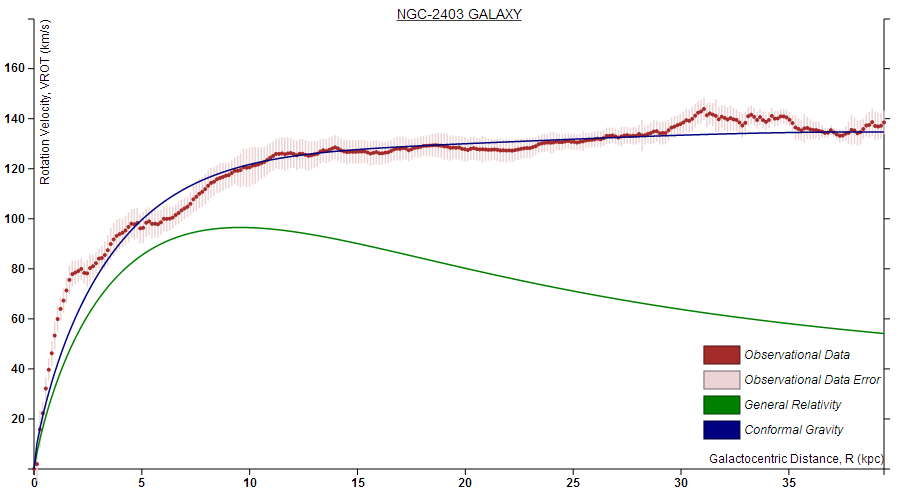
\includegraphics[width=3in, frame]{NGC-2403-PLOT}
\caption{The plotted GR and CR models vs. the observational data for NGC-2403.}
\label{ngc2403plot}
\end{figure}

When viewing a model in RoCS side by side with the simulated observational data, it's clear to see where the velocity inconsistencies arise within the modeled galaxies. The biggest difference is when the data is compared to the GR prediction as seen in Figure \ref{ngc2403gr}.

\begin{figure}[h!]
\centering
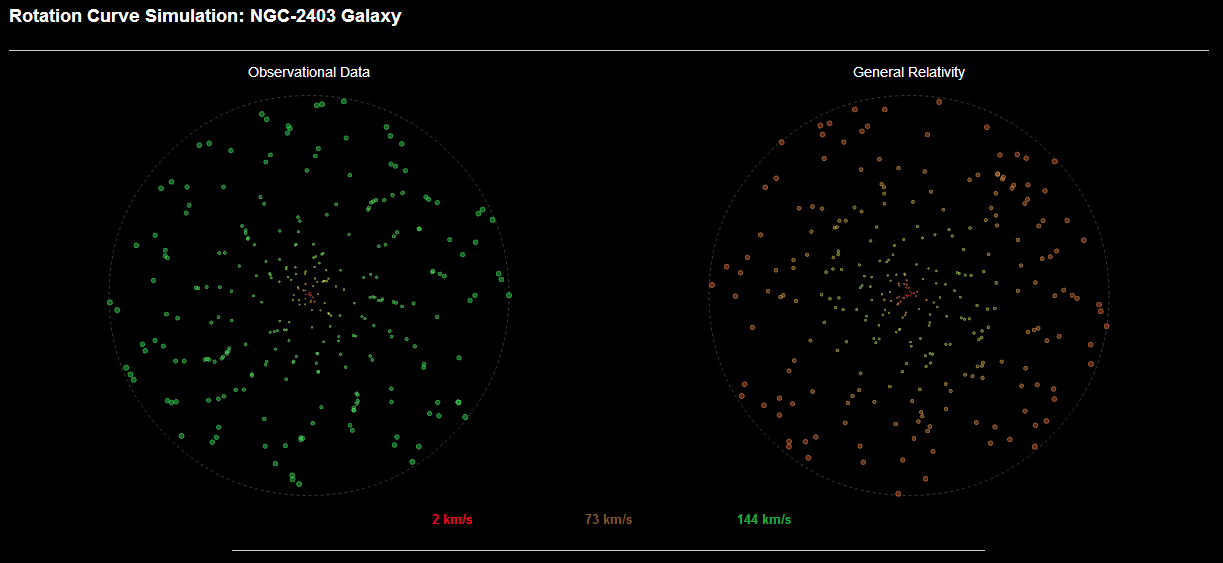
\includegraphics[width=3.5in]{NGC-2403-GR}
\caption{The simulated observational data verses the GR model for NGC-2403.}
\label{ngc2403gr}
\end{figure}

The inner parts of the galaxy seems to match the data. But about half way out, the velocity starts to slow down as described by the GR prediction, and the data stays uniform. As an alternative, the CG prediction for NGC-2403 matches clearly with the observational data in Figure \ref{ngc2403cg}.

\begin{figure}[h!]
\centering
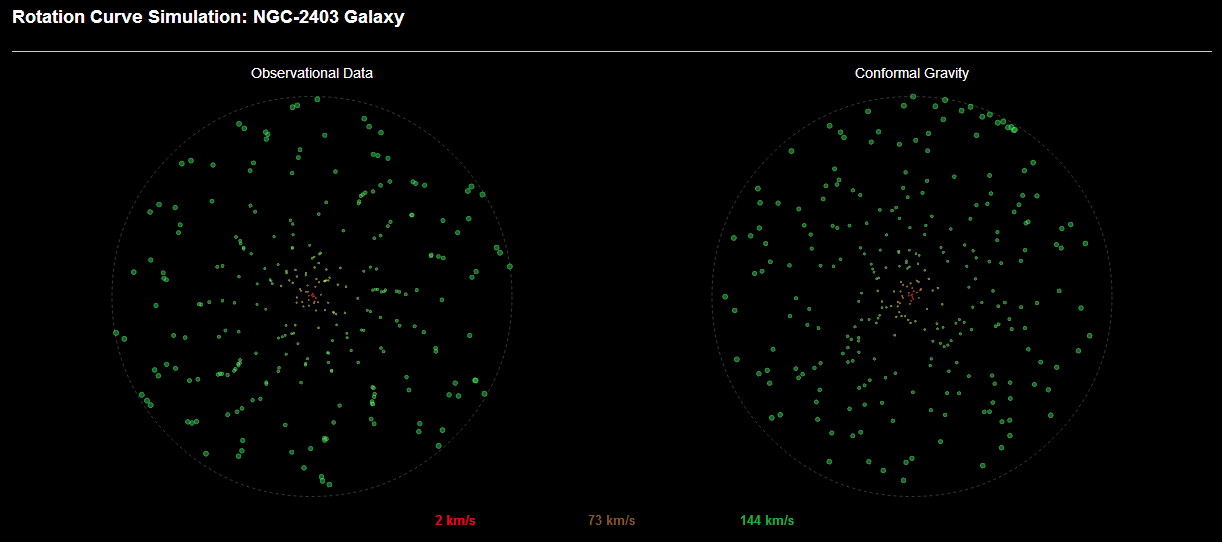
\includegraphics[width=3.5in]{NGC-2403-CG}
\caption{The simulated observational data vs. the CG model for NGC-2403.}
\label{ngc2403cg}
\end{figure}
 \newpage

\section{Conclusion}
The hope is that astronomers will use SOCM to upload observational data in one central location. Astrophysicists then can use RoCM to test that data against several galactic models to finally understand the dynamics of galaxies. 

	 We are pleased to announce that SOCM is open to the public at socm.herokuapp.com, where users can now view our database of collected measurements and developers may use our API endpoints to use in their own endeavors. RoCM is hosted online and can be found at rotationcurve.herokuapp.com. Each project is a contribution to the open source community and can be found here: https://github.com/RoCMSOCM



\section*{Acknowledgment}

We would like to thank Dr. James G. O’Brien for his work on the rotation curve problem using conformal gravity. The data mining he endured during his Ph.D process was an example of when SOCM could have been used and influenced the development of RoCM. His work impacted the successful outcome of this project. 

We would also like to thank Patrick McGee and David Miller for their extreme help building the SOCM database.



\bibliographystyle{abbrv}
\bibliography{citations}


\begin{figure*}[!t]
\centering
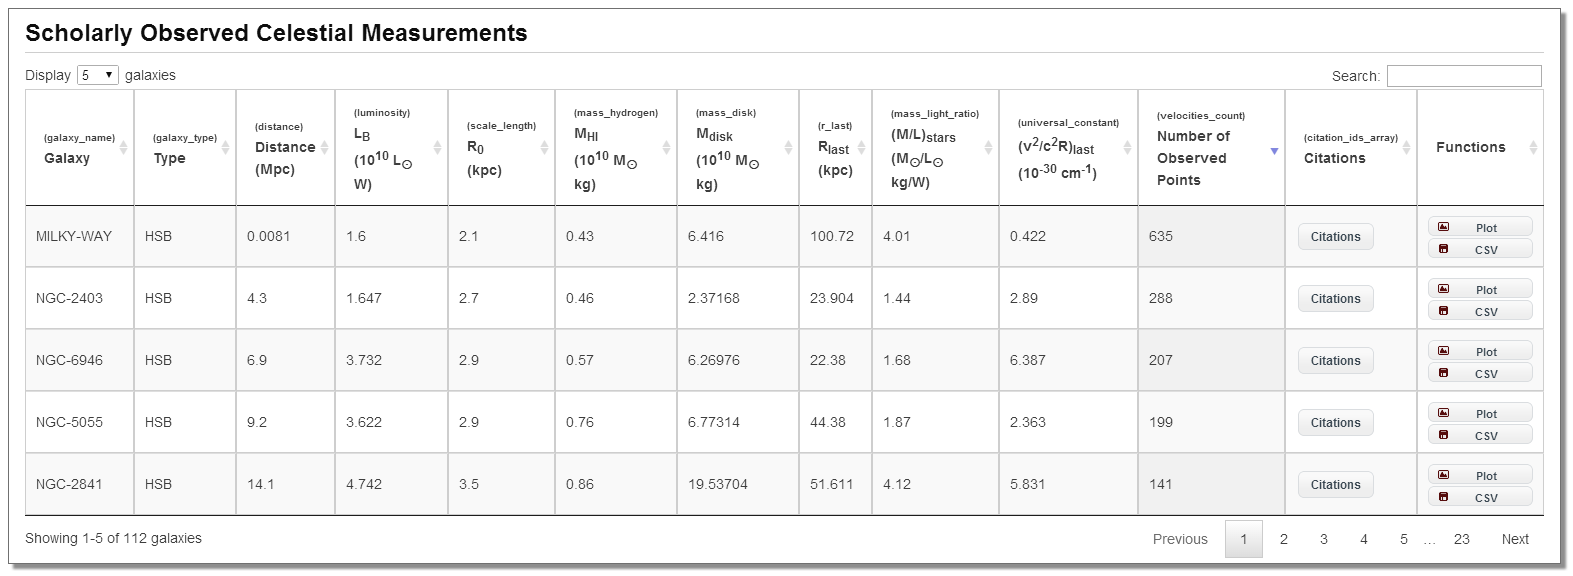
\includegraphics[width=\textwidth]{socmtable2}
\caption{The SOCM table where you can access all the galactic data.}
\label{socm_fig}
\end{figure*}

\newpage
% Appendi
\begin{appendices}

\section{Parameter Short Name Associations in RoCM} \label{short_name}
% RoCM parameter association
\begin{table}[h]

	\centering
	\normalsize
	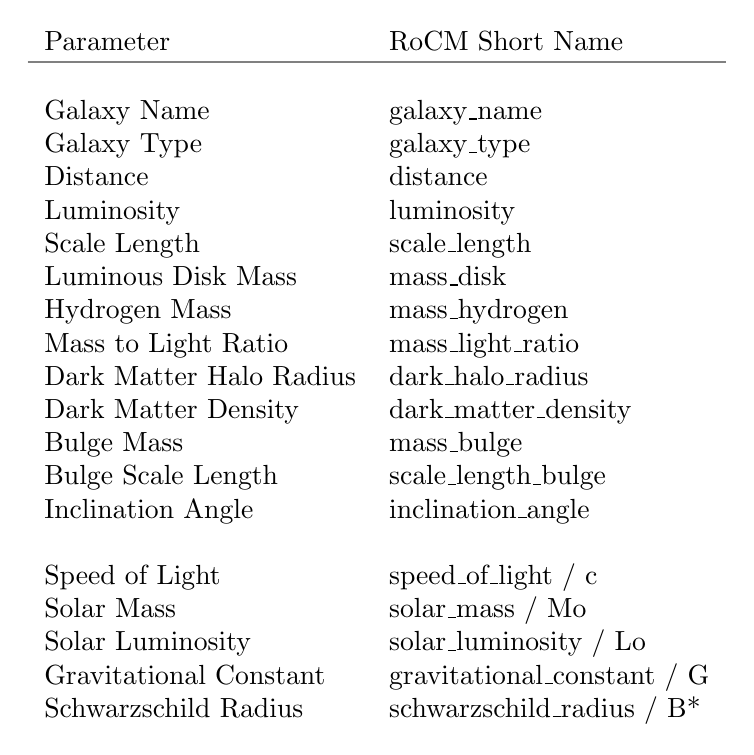
\begin{tikzpicture}
	\node[fill=white,inner sep=0pt] 
	{
		\begin{tabular}{ l l }
		Parameter \ \ \ \ \ \ \ \ \ \ \ \ \ \ \ \ \ \ \ & RoCM Short Name \\
		\arrayrulecolor{gray}\hline
		\arrayrulecolor{gray}\hline
		&\\
		Galaxy Name & galaxy\_name \\
		Galaxy Type & galaxy\_type \\
		Distance & distance\\
		Luminosity & luminosity\\
		Scale Length & scale\_length\\
		Luminous Disk Mass & mass\_disk\\
		Hydrogen Mass & mass\_hydrogen\\
		Mass to Light Ratio & mass\_light\_ratio \\
		Dark Matter Halo Radius & dark\_halo\_radius \\
		Dark Matter Density & dark\_matter\_density \\
		Bulge Mass & mass\_bulge \\
		Bulge Scale Length & scale\_length\_bulge \\
		Inclination Angle & inclination\_angle \\		
		&\\
		Speed of Light & speed\_of\_light / c \\
		Solar Mass & solar\_mass / Mo \\
		Solar Luminosity & solar\_luminosity / Lo \\
		Gravitational Constant & gravitational\_constant / G \\
		Schwarzschild Radius & schwarzschild\_radius / B* 
		\end{tabular}
	};
	\end{tikzpicture}
\end{table}

\end{appendices}

\begin{figure*}[h!]
\centering
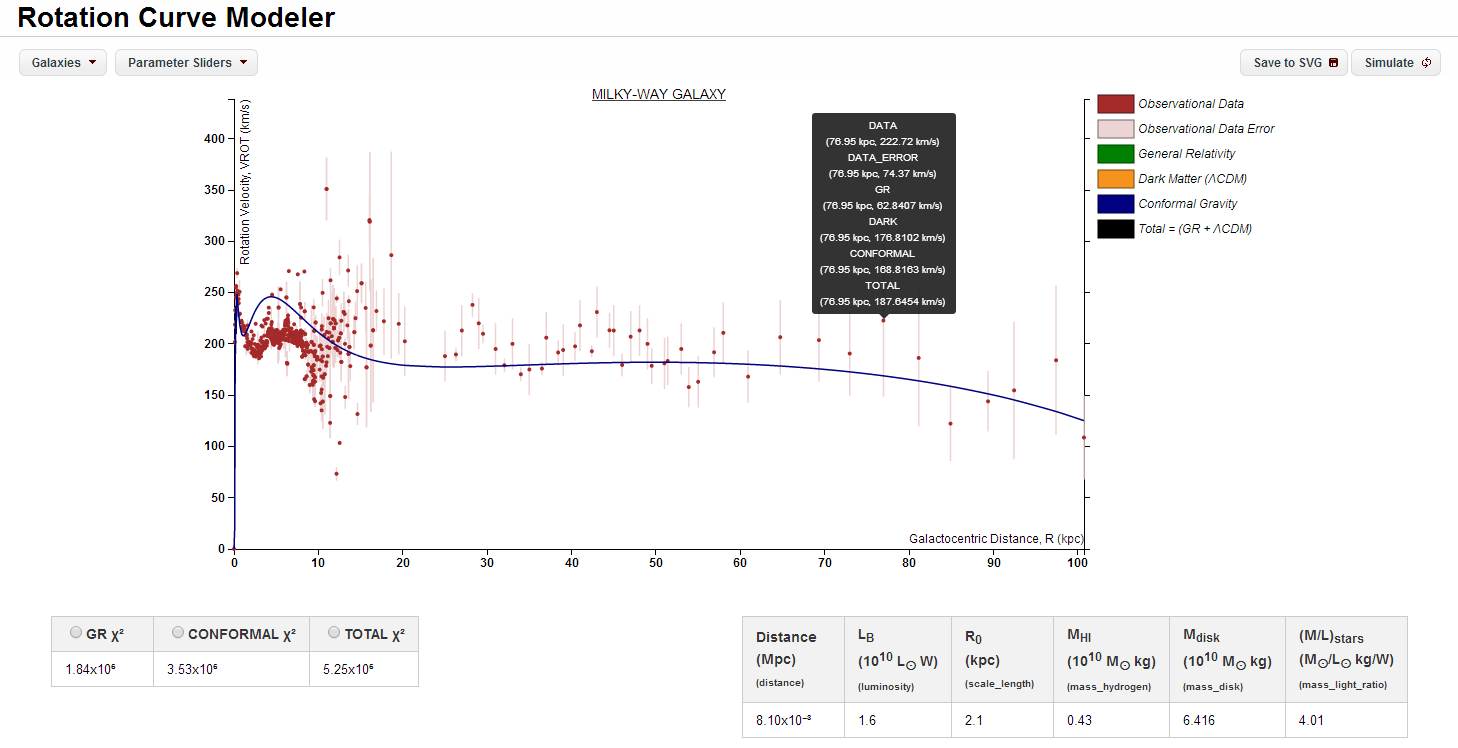
\includegraphics[width=0.95\textwidth, frame,trim = -1cm -1cm -1cm -1cm, clip]{rocm_screenshot2}
\caption{The main RoCM page where users can plot the specified galaxy (the Milky Way galaxy is shown)}
\label{rocm_fig}
\end{figure*}


\begin{figure*}[h!]
\centering
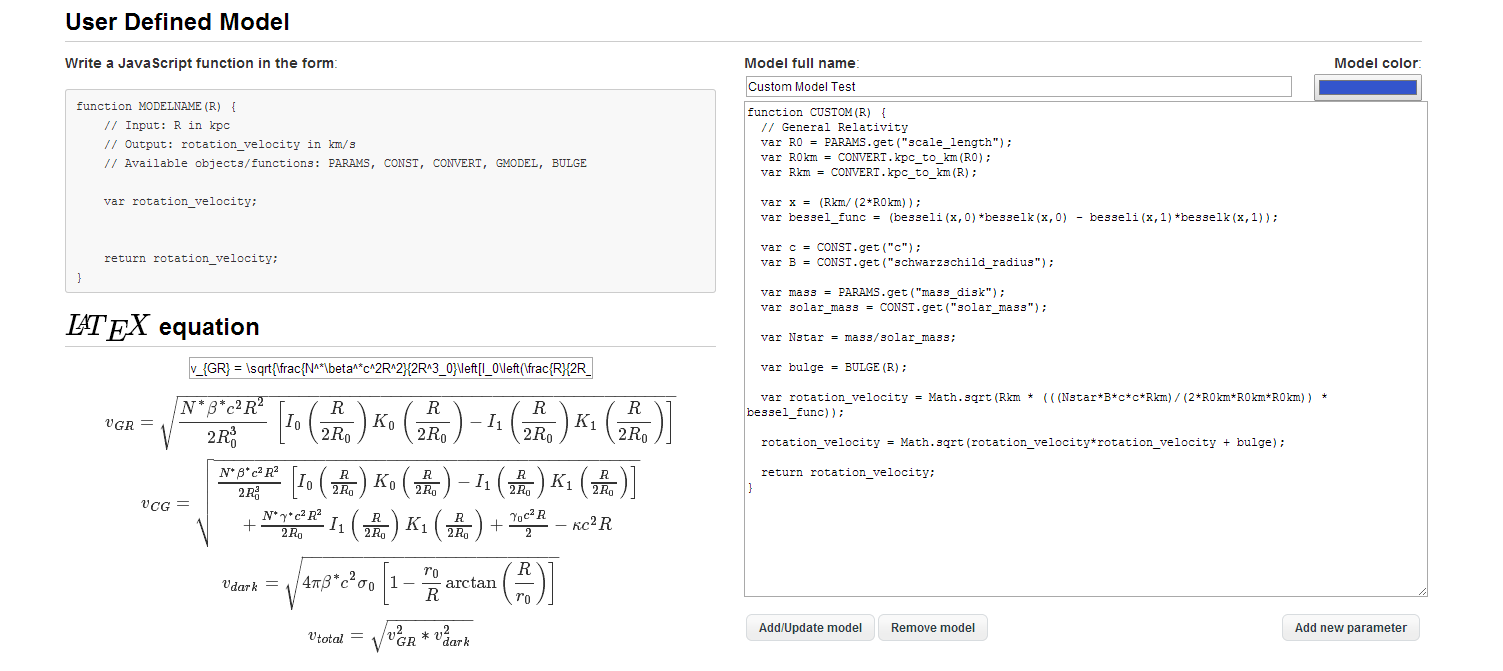
\includegraphics[width=0.95\textwidth, frame]{udm2}
\caption{The User Defined Model workbench in RoCM}
\label{udm}
\end{figure*}


\end{document}